% !TeX program = pdflatex
% Build: latexmk -pdf mainv1.tex (replace with this file's name).
\documentclass[a4paper,11pt]{article}
\usepackage{jheppub}
\usepackage{mathtools,bm}
\usepackage{orcidlink}
\allowdisplaybreaks[1]

% General-purpose commands from the FEC manuscripts.
% physics supplies bra, ket, braket, dyad, matrixel, expval,
% abs, norm, comm, acomm, dv, pdv, dd, and trace commands.
\usepackage{physics}
% Keep \sec for the trigonometric function and \pb for Poisson brackets.
\newcommand{\secref}[1]{Sec.~\ref{#1}}
\newcommand{\fig}[1]{Fig.~\ref{#1}}
\newcommand{\figs}[2]{Figs.~\ref{#1} and~\ref{#2}}
\newcommand{\eq}[1]{Eq.~\eqref{#1}}
\newcommand{\eqs}[2]{Eqs.~\eqref{#1} and~\eqref{#2}}
\newcommand{\eqss}[3]{Eqs.~\eqref{#1}~\eqref{#2} and~\eqref{#3}}
\newcommand{\refcite}[1]{Ref.~\cite{#1}}
\newcommand{\refs}[1]{Refs.~\cite{#1}}
\newcommand*{\Scale}[2][4]{\scalebox{#1}{\ensuremath{#2}}}

\newcommand{\pp}[1]{\left(#1\right)}
\newcommand{\bb}[1]{\left[#1\right]}
\newcommand{\cc}[1]{\left\{#1\right\}}
\newcommand{\vv}[1]{\left\langle #1 \right\rangle}
\newcommand{\bigpp}[1]{\big(#1\big)}
\newcommand{\bigbb}[1]{\big[#1\big]}
\newcommand{\bigcc}[1]{\big\{#1\big\}}
\newcommand{\bigvv}[1]{\big\langle #1 \big\rangle}
\newcommand{\Bigpp}[1]{\Big(#1\Big)}
\newcommand{\Bigbb}[1]{\Big[#1\Big]}
\newcommand{\Bigcc}[1]{\Big\{#1\Big\}}
\newcommand{\Bigvv}[1]{\Big\langle #1 \Big\rangle}
\newcommand{\biggpp}[1]{\bigg(#1\bigg)}
\newcommand{\biggbb}[1]{\bigg[#1\bigg]}
\newcommand{\biggcc}[1]{\bigg\{#1\bigg\}}
\newcommand{\biggvv}[1]{\bigg\langle #1 \bigg\rangle}

\newcommand{\iv}[1]{\left[#1\right]}
\newcommand{\bigiv}[1]{\big[#1\big]}
\newcommand{\biggiv}[1]{\bigg[#1\bigg]}

\newcommand{\beq}[1][]{\begin{equation}\if\relax\detokenize{#1}\relax\else\label{#1}\fi}
\newcommand{\eeq}{\end{equation}}
\newcommand{\bse}[1][]{\begin{subequations}\if\relax\detokenize{#1}\relax\else\label{#1}\fi}
\newcommand{\ese}{\end{subequations}}
\newcommand{\nn}{\nonumber}

\newcommand{\wt}[1]{\widetilde{#1}}
\newcommand{\GeV}{\mathrm{GeV}}
\newcommand{\pbu}{\mathrm{pb}}
\newcommand{\MS}{\overline{\mathrm{MS}}}
\newcommand{\LQCD}{\Lambda_{\mathrm{QCD}}}
\newcommand{\lo}{{[0]}}
\newcommand{\nlo}{{[1]}}

% Add your own macros here.

\title{Calculation with Spins}
\author{Shu-Tao Zhang\,\orcidlink{0009-0009-5269-2364}}
\affiliation{School of Physics, Peking University, Beijing 100871, China}
\emailAdd{shutaozhang@pku.edu.cn}
\date{\today}
\abstract{%
% State the question, approach, main result, and domain of validity.
Write your abstract here.
}

\begin{document}
\maketitle
\flushbottom

\section{\texorpdfstring{$e^+e^-\to\mu^+\mu^-$}{e+e- to mu+mu-} helicity benchmark}
\label{sec:ee-benchmark}

\subsection{Kinematics}
\label{sec:setup}
% Define the observable, conventions, scales, and assumptions.
In this note, we calculate the helicity amplitudes for the process $e^+ e^- \to \mu^+ \mu^-$, including the effects of transverse spin polarization. We adopt the spinor helicity formalism and follow the conventions outlined in Peskin book. 
The kinematics are summarized as follows, the incoming electron and positron have momenta $p_1$ and $p_2$, respectively, while the outgoing muon and antimuon have momenta $k_1$ and $k_2$. The explicit expressions for the momentum are given by:
\begin{align}
    p_1^\mu &= \frac{\sqrt{s}}{2} (1, 0, 0, 1), \\
    p_2^\mu &= \frac{\sqrt{s}}{2} (1, 0, 0, -1), \\
    k_1^\mu &= \frac{\sqrt{s}}{2} (1, \sin\theta, 0, \cos\theta), \\
    k_2^\mu &= \frac{\sqrt{s}}{2} (1, -\sin\theta, 0, -\cos\theta),
\end{align}
While the Mandelstam variables are defined as:
\begin{align}
    s &= (p_1 + p_2)^2, \\
    t &= (p_1 - k_1)^2 = \frac{s}{2}\pp{\cos\theta-1}, \\
    u &= (p_1 - k_2)^2 = \frac{s}{2}\pp{-\cos\theta-1},
\end{align}
with $s + t + u = 0$ in our massless approximation.

\subsection{Helicity and chirality}
Now we define the spinor helicity conventions. For simplicity we consider the massless case, while the massive case can be left as future investigation.
In the Appendix B of Peskin book, the spinors are:
\begin{align}
    u_\lambda(p) &= \begin{pmatrix} \sqrt{p\cdot\sigma} \, \xi_\lambda \\ \sqrt{p\cdot\bar{\sigma}} \, \xi_\lambda \end{pmatrix}, \\
    v_\lambda(p) &= \begin{pmatrix} \sqrt{p\cdot\sigma} \, \eta_\lambda \\ -\sqrt{p\cdot\bar{\sigma}} \, \eta_\lambda \end{pmatrix},
\end{align}
With the spinors $\xi_\lambda$ and $\eta_\lambda$ defined in Eq.~(3.134)
\begin{align}
    \xi_+(p) &= \begin{pmatrix} \cos\frac{\theta}{2} \\ e^{i\phi}\sin\frac{\theta}{2} \end{pmatrix}, \nn\\
    \xi_-(p) &= \begin{pmatrix} -e^{-i\phi}\sin\frac{\theta}{2} \\ \cos\frac{\theta}{2} \end{pmatrix}, \nn\\
    \eta_+(p) &= \xi_-(p),  \nn\\
    \eta_-(p) &= -\xi_+(p),
\end{align}
which lead to
\begin{align}
    u_\pm(p) &= \begin{pmatrix} \sqrt{E \mp \abs{\bm p}} \, \xi_\pm \\ \sqrt{E \pm \abs{\bm p}} \, \xi_\pm \end{pmatrix}, \\
    v_\pm(p) &= \begin{pmatrix} \sqrt{E \pm \abs{\bm p}} \, \eta_\pm \\ -\sqrt{E \mp \abs{\bm p}} \, \eta_\pm \end{pmatrix}.
\end{align}
Here $\theta$ and $\phi$ are the polar and azimuthal angles of the momentum $p$ in the spherical coordinate system, which should be separated from the kinematics.
The helicity basis here means the spin \textcolor{blue}{quantization axis} is aligned with the momentum direction, while in \textcolor{blue}{a fixed-axis basis the spin quantization axis is chosen along a fixed direction such as} the $z$-axis.

One should note that the spinor helicity allow an overall arbitrary phase. However, during the calculation, one should fix the phase convention to avoid ambiguity for defining the transverse spin.
% For the fermion spinors $u$, one have a natural helicity operator definition, which is
% \begin{align}
    
% \end{align}

Finally, we demonstrate the relation of the spinor helicity and the chirality.
\begin{align}
    P_R u_+(p) &= u_+(p), \quad P_L u_-(p) = u_-(p), \quad \gamma_5 u_{L/R}(p) = \mp u_{L/R}(p), \\
    P_R v_-(p) &= v_-(p), \quad P_L v_+(p) = v_+(p), \quad \gamma_5 v_{L/R}(p) = \mp v_{L/R}(p).
\end{align}

\subsection{Transverse spin and helicity density matrices}
\begin{sloppypar}
The derivation of the transverse spin of a fermion can be found in hep-ph/0104283, Eq.~(2.2.6). Normally we don't use the transverse polarized spinor directly, still, we summarize the main results here.
\end{sloppypar}
\begin{align}
    u^x_+(p) &= \frac{1}{\sqrt{2}}\bb{u_+(p) + u_-(p)}, \\
    u^x_-(p) &= \frac{1}{\sqrt{2}}\bb{u_+(p) - u_-(p)}, \\
    u^y_+(p) &= \frac{1}{\sqrt{2}}\bb{u_+(p) + i u_-(p)}, \\
    u^y_-(p) &= \frac{1}{\sqrt{2}}\bb{u_+(p) - i u_-(p)}, \\
    v^x_+(p) &= \frac{1}{\sqrt{2}}\bb{v_+(p) + v_-(p)}, \\
    v^x_-(p) &= \frac{1}{\sqrt{2}}\bb{v_+(p) - v_-(p)}, \\
    v^y_+(p) &= \frac{1}{\sqrt{2}}\bb{v_+(p) - i v_-(p)}, \\
    v^y_-(p) &= \frac{1}{\sqrt{2}}\bb{v_+(p) + i v_-(p)}.
\end{align}
The last two equations comes from the fact that charge conjugation involves a conjugation of the spinor, which flips the sign of the imaginary unit $i$.
Please note that all these component allows an overall arbitrary phase, what is important is the relative phase of $u_+$ and $u_-$.
Therefore, in some other references, one may find different overall phase conventions, don't be surprised.

A more convenient way to think about the transverse spin is to use the density matrix formalism, which is discussed in hep-ph/0104283, Eq.~(2.3.4). The density matrix of a fermion with transverse spin can be expressed as:
\begin{align}
    \rho = \tfrac 1 2 \begin{pmatrix}
        1+s_z \quad s_x-is_y\\
        s_x+is_y \quad 1-s_z
    \end{pmatrix}
    \propto \mathcal{H}_{\lambda\lambda'} = \begin{pmatrix}
        \mathcal{H}_{++} \quad \mathcal{H}_{+-}\\
        \mathcal{H}_{-+} \quad \mathcal{H}_{--}
    \end{pmatrix},
\end{align}
where the $\mathcal{H}_{\lambda\lambda'}$ is the interference term of the helicity amplitudes, with the observed fermion spin indices open.
In this expression, the overall phase in the transverse polarized spinor is irrelevant, however, the relative phase between $u_+$ and $u_-$ still counts. For example, if we add a phase factor $e^{i\bar\phi}$ to \textcolor{blue}{the basis spinor} $u_+$ \textcolor{blue}{while keeping the physical spin fixed}, then the density matrix becomes:
\begin{align}
    \rho = \tfrac 1 2 \begin{pmatrix}
        1+s_z \qquad e^{-i\bar\phi}(s_x-is_y)\\
        e^{i\bar\phi}(s_x+is_y) \qquad 1-s_z
    \end{pmatrix}.
\end{align}

Finally, one can calculate

\subsection{Tree-level QED amplitudes}
\label{sec:derivation}
% Derive the result and explain the approximations.
In this section, we calculate the helicity amplitudes for the process $e^+ e^- \to \mu^+ \mu^-$, which is an easy example for the future calculation.
Though many much more effective methods exist, we use the easiest one. We first write down the explicit expressions for the spinors, then we substitute them into the Feynman ampltiudes.

% --------------- Feynman Diagram ---------------
\begin{figure}[htbp]
    \centering
    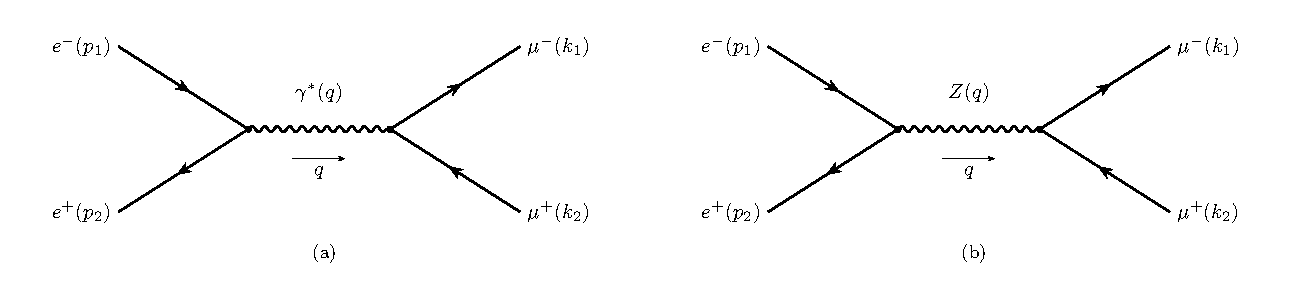
\includegraphics[width=\textwidth]{ee_to_mumu_tree.pdf}
    \caption{Feynman diagrams involving QED and EW interactions}
    \label{fig:feynman-diagrams}
\end{figure}
% ---------------

Consider the QED process first and leave all the helicity indices open, we get:
\begin{align}
    i\mathcal{M}_{\lambda_1\lambda_2\lambda_3\lambda_4} &= \bar{v}_{\lambda_2}(p_2) (-ie\gamma^\mu) u_{\lambda_1}(p_1) \frac{-i g_{\mu\nu}}{s} \bar{u}_{\lambda_3}(k_1) (-ie\gamma^\nu) v_{\lambda_4}(k_2).
\end{align}

Substituting the explicit massless spinors gives the helicity amplitudes below.
To fix their relative phases, we use the two-component spinors defined above and choose the polar and azimuthal angles
\begin{align}
    (\theta_{p_1},\phi_{p_1}) &= (0,0), &
    (\theta_{p_2},\phi_{p_2}) &= (\pi,\pi), \nn\\
    (\theta_{k_1},\phi_{k_1}) &= (\theta,0), &
    (\theta_{k_2},\phi_{k_2}) &= (\pi-\theta,\pi).
\end{align}
The azimuth at the south pole is a spinor phase convention, even though it does not affect the momentum.
With rows labeled by $(\lambda_1,\lambda_2)$ and columns by $(\lambda_3,\lambda_4)$, the entries are $\mathcal{M}_{\lambda_1\lambda_2\lambda_3\lambda_4}/e^2$, rather than $i\mathcal{M}/e^2$:
\begin{equation}
\label{eq:qed-helicity-amplitudes}
    \begin{array}{c|cccc}
        (\lambda_1,\lambda_2)\backslash(\lambda_3,\lambda_4)
            & ++ & +- & -+ & -- \\ \hline
        ++  & 0 & 0 & 0 & 0 \\
        +-  & 0 & -(1+\cos\theta) & 1-\cos\theta & 0 \\
        -+  & 0 & 1-\cos\theta & -(1+\cos\theta) & 0 \\
        --  & 0 & 0 & 0 & 0
    \end{array}.
\end{equation}
Only opposite-helicity fermion--antifermion pairs contribute in the massless limit.
Summing over final helicities and averaging over initial helicities reproduces the unpolarized QED result,
\begin{equation}
\label{eq:qed-helicity-spin-sum}
    \frac{1}{4}\sum_{\lambda_1,\lambda_2,\lambda_3,\lambda_4}
    \left|\mathcal{M}_{\lambda_1\lambda_2\lambda_3\lambda_4}\right|^2
    = e^4\left(1+\cos^2\theta\right),
\end{equation}
which also agrees with an independent Dirac-trace calculation.

\section{Collinear factorization for dihadron SIDIS}
\label{sec:sidis-factorization}

\subsection{Kinematics}
We investigate the SIDIS process, with two hadron in the final state.

\begin{equation}
    e^-(\ell)+p(P)\to e^-(\ell')+(h_1+h_2)(P_h=P_1+P_2)+X .
    \label{eq:sidis-process}
\end{equation}
In the QED LO approximation, the process is mediated by a virtual photon $\gamma^*(q)$, with $q=\ell-\ell'$ and $Q^2=-q^2$.
The hadron level Lorentz invariants are usually chosen as

\begin{equation}
    s=2P\cdot\ell,
    x_B=\frac{Q^2}{2P\cdot q}, y=\frac{P\cdot q}{P\cdot\ell},
    z_h=\frac{P\cdot P_h}{P\cdot q},Q^2=x_By\,s.
    \label{eq:sidis-kinematics}
\end{equation}

Here $P_h = P_1 + P_2$, while for the single hadron production process, it is simply the observed hadron's momentum, so the discussion is a simple generalization of the single hadron case.
%
Dihadron observables are further defined with the relative momentum $R=(P_1-P_2)/2$ and the invariant mass $M_h^2=P_h^2$.

We don't bother to define the light-cone projections, the reader can easily access with AI.

For the factorization to be valid, the hierarchy $Q\gg M_h,\Lambda_{\rm QCD}$ is required.
Another interesting point is the hierarchy of $M_h$ and $\Lambda_{\rm QCD}$, the conclusion is that, SCET told us that a jet function can be defined for both $M_h\sim\Lambda_{\rm QCD}$ and $M_h\gg\Lambda_{\rm QCD}$. However, the jet function itself can be further factorized when $M_h\gg\Lambda_{\rm QCD}$, which involves the methods of operation product expansion (OPE). This is beyond the scope of this note.

\subsection{Factorization and its convolution structure}
A common convolution structure of factorization is as follows, with no polarization dependence at this stage:
\begin{equation}
    \begin{aligned}
        \frac{\dd\sigma^{UU}}{\dd\Pi(\ell')\,\dd\Pi(\hat P_h)\,\dd M_h}
        &\overset{L.P.}{=} \sum_{a,b}\int_0^1\dd x\, f_1^a(x;\mu)
                  \int_0^1\frac{\dd\xi}{\xi^2}\,D_1^b(\xi,M_h;\mu)\,
                  \frac{\dd\widehat\sigma^{UU}_{ba}}
                       {\dd\Pi(\ell')\,\dd\Pi(\widehat k)}\\
        &= \frac{1}{2s}\sum_{a,b}\int_0^1\frac{\dd x}{x}
                  \int_0^1\frac{\dd\xi}{\xi^2}\,
                  f_1^a(x;\mu)\,{\cal H}^{UU}_{ba}(xP, P_h/\xi)\,D_1^b(\xi,M_h;\mu).
    \end{aligned}
    \label{eq:sidis-unpolarized-invariant-convolution}
\end{equation}
Here $$\dd \Pi(k) = \frac{\dd^4 k}{(2\pi)^3} \delta(k^2) \theta(k^0) = \frac{\dd^3k}{(2\pi)^3 2k^0}$$ is the Lorentz Invariant Phase Space element. The $\hat k$ labels a momentum that is approximately massless. L.P. means the leading power approximation in the $1/P^+$ expansion.
The upper case $UU$ means unpolarized beam and unpolarized target, while the lower case $a,b \in \{q,\bar q,g\}$ labels the parton flavors.
$\hat \sigma$ means the partonic cross section, and ${\cal H}$ is the hard scattering coefficient or the amplitudes squared, 

\begin{equation}
    \begin{aligned}
        {\cal H}_{ba}(xP,P_h/\xi)
        &=\sum_X\int\dd\Pi_X\, (2\pi)^4
          \delta^{(4)}\bigl(\ell+xP-\ell'-P_h/\xi-P_X\bigr)\\
        &\quad\times
          \abs{M\bigl(e^-(\ell)+a(xP)\to e^-(\ell')+
                      b(P_h/\xi)+X\bigr)}^2 .
    \end{aligned}
    \label{eq:sidis-hard-scattering}
\end{equation}


For the nonperturbative functions $f,D$, they have number density interpretation, which is defined as the number of partons per unit momentum fraction.
In this case, the naive convolution should be 
$$
\sigma = \int \dd x \, \dd \xi \, f(x) \hat \sigma(x,\xi) D(\xi) ,
$$
However, due to the phase space Jacobian and the partonic flux factor, the convolution structure is modified to the form in \eqref{eq:sidis-unpolarized-invariant-convolution}.
The weight $\frac{1}{\xi^2}$ comes from the phase space Jacobian from $\dd\Pi(\hat k)$ to $\dd\Pi(\hat P_h)$, by noting that $\hat P_h = \xi \hat k$ and the mass dimension of $[d\Pi]=2$.
The weight $\frac{1}{x}$ comes from the partonic flux factor $F=\frac{1}{2\hat s}$ and $\hat s = x s$.
Therefore, a general factorization structure involves this typical weight that is seen everywhere.

\subsection{Phase space simplification}

Now we try to simplify the phase space to independent Lorentz invariants in \eqref{eq:sidis-kinematics}.
First we introduce the Sudakov decomposition to convert the LIPS to several Lorentz invariants.
First people choose two light-cone vectors $n$ and $\bar n$, with $n^2=\bar n^2=0$ and operate the decomposition exactly same as the light cone coordinates: $K = a n + b \bar n + K_\perp$.
Then one find $d^4K = (n\cdot \bar n) \dd a \dd b \dd^2 K_\perp$ and $K^2 = 2(n\cdot \bar n) ab + K_\perp^2$.
The value of $a,b$ can be read off by dotting the opposite light-cone vectors, $$
a = \frac{K \cdot \bar n}{n \cdot \bar n}, \quad b = \frac{K \cdot n}{n \cdot \bar n}.
$$

We now take outgoing electron as an example.
\begin{equation}
    \ell'=\alpha\ell+\beta P+\ell'_\perp,\qquad
    \alpha=\frac{\ell'\cdot P}{\ell\cdot P}=1-y,\qquad \beta=\frac{\ell'\cdot \ell}{\ell\cdot P}=x_By,\qquad
    -\ell_\perp^{\prime\,2}=s\alpha\beta .
    \label{eq:sidis-lepton-sudakov}
\end{equation}
The we have:
\begin{equation}
    \begin{aligned}
        \dd\Pi(\ell')
        &=\frac{\ell\cdot P}{2(2\pi)^3}\,\dd\alpha\,\dd\beta\,\dd\psi
          \int_0^\infty\dd\bm\ell_\perp^{\prime\,2}\,
          \delta\bigl(s\alpha\beta-\bm\ell_\perp^{\prime\,2}\bigr)\\
        &=\frac{s}{4(2\pi)^3}
          \abs{\frac{\partial(\alpha,\beta)}{\partial(x_B,y)}}\,
          \dd x_B\,\dd y\,\dd\psi
          =\frac{ys}{16\pi^2}\,\dd x_B\,\dd y\,\frac{\dd\psi}{2\pi}.
    \end{aligned}
    \label{eq:sidis-lepton-phase-space}
\end{equation}

For the total momentum $P_h$, we choose light-cone basis $q+x_BP$ and $P$. Then we get the following Sudakov decomposition,
\begin{equation}
    \begin{aligned}
        P_h^\mu&=z_h(q+x_BP)^\mu+\beta_h P^\mu+P_{hT}^\mu,\quad 2q\cdot P = Q^2/x_B\\
        P_{hT}\cdot P&=P_{hT}\cdot q=0,\qquad
        \bm P_{hT}^{\,2}=-P_{hT}^2,\qquad
        \beta_h=\frac{x_B(M_h^2+\bm P_{hT}^{\,2})}{z_hQ^2}.
    \end{aligned}
    \label{eq:sidis-pair-sudakov}
\end{equation}
Here we choose the transverse momentum to survive in the phase space integral, therefore the coefficient $\beta_h$ is expected to eliminate by the mass-shell condition $P_h^2=M_h^2$.
Then the LIPS is given by
\begin{equation}
    \begin{aligned}
        \dd\Pi(P_h)
        &=\frac{Q^2}{2x_B}\frac{\dd z_h\,\dd^2\bm P_{hT}}{(2\pi)^3}
          \int\dd\beta_h\,
          \delta\left(\frac{z_h\beta_h Q^2}{x_B}-\bm P_{hT}^{\,2}-M_h^2\right)
          \theta(P_h^0)\\
        % =\frac{\dd z_h\,\dd^2\bm P_{hT}}{2(2\pi)^3z_h}
        &=\frac{\dd z_h\,\dd\bm P_{hT}^{\,2}}{16\pi^2z_h}
          \frac{\dd\phi}{2\pi}.
    \end{aligned}
    \label{eq:sidis-pair-invariant-phase-space}
\end{equation}

For the integration of $\dd\Pi(\hat P_h)$, one simply set $M_h=0$ in equation~\eqref{eq:sidis-pair-sudakov} and \eqref{eq:sidis-pair-invariant-phase-space}, and the final result is the same as the above.

Multiplying the two measures gives the Jacobian for the left-hand
side of \eqref{eq:sidis-unpolarized-invariant-convolution},
\begin{equation}
    \begin{aligned}
        \dd\Pi(\ell')\,\dd\Pi(\hat P_h)\,\dd M_h
        &=\frac{ys}{256\pi^4 z_h}\,
        \dd x_B\,\dd y\,\dd z_h\,\dd\bm P_{hT}^{\,2}\,\dd M_h\,
        \frac{\dd\psi}{2\pi}\frac{\dd\phi}{2\pi},
    \end{aligned}
    \label{eq:sidis-reduced-phase-space}
\end{equation}
Here we have to choose the reference axis to define two azimuthal angles $\psi$ and $\phi$. For the unpolarized initial state, the $\psi$ dependence should be trivial, therefore we simply integrate and drop it.
While the $\phi$ dependence is usually chosen in the so called Breit frame, which is defined by boosting the frame so that
$$
q = (0,0,0,-Q), \quad P = \frac{Q}{2x_B}(1,0,0,1), \quad \ell^\mu = \frac{Q}{2y}\left(2 - y,\; 2\sqrt{1 - y},\; 0,\; -y\right).
$$




\clearpage
\section{Spin-dependent dihadron SIDIS}
\label{sec:sidis-formulae}

\subsection{Spin-resolved number densities}

\begin{equation}
    \begin{aligned}
        \hat{\bm z}_e&=\frac{\bm\ell}{|\bm\ell|},\qquad
        \hat{\bm z}_a=\frac{\bm P}{|\bm P|},\qquad
        \hat{\bm z}_b=\frac{\bm P_h}{|\bm P_h|},\\
        \hat{\bm y}_e&=\frac{\bm q\times\bm\ell}{|\bm q\times\bm\ell|},\qquad
        \hat{\bm y}_j=\frac{\hat{\bm z}_j\times\bm\ell}
                            {|\hat{\bm z}_j\times\bm\ell|},\quad j=a,b,\\
        \hat{\bm x}_j&=\hat{\bm y}_j\times\hat{\bm z}_j,\qquad j=e,a,b
        \qquad(\mathrm{Breit}).
    \end{aligned}
    \label{eq:sidis-spin-axes}
\end{equation}
\begin{equation}
    \begin{aligned}
        \bm R_T&=\bm R-(\bm R\cdot\hat{\bm z}_b)\hat{\bm z}_b,\\
        \hat{\bm R}_T&=\hat{\bm x}_b\cos\phi_R+\hat{\bm y}_b\sin\phi_R,\qquad
        \hat{\bm n}_R=\hat{\bm z}_b\times\hat{\bm R}_T.
    \end{aligned}
    \label{eq:sidis-azimuths}
\end{equation}
\begin{equation}
    \rho(\bm s)=\frac{\mathbf 1+\bm s\cdot\bm\sigma}{2},\qquad
    \rho_e=\rho(\bm s_e),\qquad
    \bm\sigma_T=(\sigma_x,\sigma_y),\qquad \abs{\bm s}\leq 1 .
    \label{eq:sidis-spin-projector}
\end{equation}
\begin{equation}
    \begin{aligned}
        {\cal F}_a(x,S;\mu)
        &=\frac{1}{2}\left[f_1^a(x;\mu)\,\mathbf 1
            +S_Lg_1^a(x;\mu)\,\sigma_z
            +h_1^a(x;\mu)\,\bm S_T\cdot\bm\sigma_T\right],\\
        S_L&=\bm S_{\rm rest}\cdot\hat{\bm z}_a,\qquad
        \bm S_T=(\bm S_{\rm rest}\cdot\hat{\bm x}_a,\,
                  \bm S_{\rm rest}\cdot\hat{\bm y}_a),\\
        \frac{\dd N_{a(\pm\hat{\bm u})/p(S)}}{\dd x}
        &=\operatorname{Tr}\!\left[\rho(\pm\hat{\bm u}){\cal F}_a\right]
        =\frac{f_1^a\pm S_Lg_1^a\,u_z\pm h_1^a\,\bm S_T\cdot\bm u_T}{2}.
    \end{aligned}
    \label{eq:sidis-spin-pdf}
\end{equation}
\begin{equation}
    \begin{aligned}
        {\cal D}_b(\xi,M_h,\phi_R;\mu)
        &=D_1^b(\xi,M_h;\mu)\,\mathbf 1
            +H_1^{\sphericalangle b}(\xi,M_h;\mu)\,\hat{\bm n}_R\cdot\bm\sigma,\\
        {\cal N}_b(\bm s_b)
        &\equiv\frac{\dd N_{h_1h_2/b(\bm s_b)}}{\dd\xi\,\dd M_h\,(\dd\phi_R/2\pi)}
         =\operatorname{Tr}\!\left[\rho(\bm s_b){\cal D}_b\right]\\
        &=D_1^b+H_1^{\sphericalangle b}
                         (s_{b,y}\cos\phi_R-s_{b,x}\sin\phi_R),\\
        \bigl(D_1^b,H_1^{\sphericalangle b}\bigr)
        &=\frac{1}{2}\bigl({\cal N}_b(\hat{\bm n}_R)+{\cal N}_b(-\hat{\bm n}_R),\,
                           {\cal N}_b(\hat{\bm n}_R)-{\cal N}_b(-\hat{\bm n}_R)\bigr).
    \end{aligned}
    \label{eq:sidis-spin-diff}
\end{equation}

\subsection{Hard helicity interference}

\begin{equation}
    \begin{aligned}
        \widehat k&=\hat P_h/\xi,\qquad a,b\in\{q,\bar q\},\\
        {\cal H}_{ba;\lambda\lambda'}^{rr';\eta\eta'}(xP,P_h/\xi)
        &=\left[\frac{1}{N_c}\sum_{X,r_f,\mathrm{colors}}
           \int\dd\Pi_X\,(2\pi)^4\delta^{(4)}(q+xP-\widehat k-P_X)\right.\\[-1pt]
        &\qquad\left.{}\times M^{ba}_{r_f\lambda X;r\eta}
                  \bigl(M^{ba}_{r_f\lambda' X;r'\eta'}\bigr)^*
          \right]_{\mathrm{ren.,\,coll.\ sub.}},\\
        {\cal H}_{ba;\lambda\lambda'}[\rho_e,{\cal F}_a]
        &=\sum_{r,r',\eta,\eta'}(\rho_e)_{rr'}({\cal F}_a)_{\eta\eta'}\,
                          {\cal H}_{ba;\lambda\lambda'}^{rr';\eta\eta'} .
    \end{aligned}
    \label{eq:sidis-hard-helicity-matrix}
\end{equation}
\begin{equation}
    \begin{aligned}
        {\cal H}_{ba}&=\frac{{\cal H}_{ba,0}}{2}
                        \bigl(\mathbf 1+\bm s_b^{\,{\cal H}}\cdot\bm\sigma\bigr),
        \qquad {\cal H}_{ba,0}=\operatorname{Tr}{\cal H}_{ba},\\
        {\cal H}_{ba,0}\bigl(s_{b,x}^{\,{\cal H}},s_{b,y}^{\,{\cal H}}\bigr)
        &=\bigl(2\operatorname{Re}{\cal H}_{ba;+-},
                -2\operatorname{Im}{\cal H}_{ba;+-}\bigr).
    \end{aligned}
    \label{eq:sidis-hard-transverse-spin}
\end{equation}

\subsection{Spin-dependent factorization}

\begin{equation}
    \begin{aligned}
        \dd\Gamma_{\rm inv}
        &=\dd\Pi(\ell')\,\dd\Pi(\hat P_h)\,\dd M_h\,\frac{\dd\phi_R}{2\pi},\\
        \frac{\dd\sigma^{(q,\bar q)}}{\dd\Gamma_{\rm inv}}
        &\overset{\rm L.P.}{=}\frac{1}{2s}\sum_{a,b=q,\bar q}
            \int_0^1\frac{\dd x}{x}\int_0^1\frac{\dd\xi}{\xi^2}
          \operatorname{Tr}\!\left[{\cal H}_{ba}[\rho_e,{\cal F}_a]\,{\cal D}_b\right],\\
        \operatorname{Tr}\!\left[{\cal H}_{ba}{\cal D}_b\right]
        &=D_1^b\,{\cal H}_{ba,0}
           -2H_1^{\sphericalangle b}\operatorname{Im}
                              \!\left[e^{i\phi_R}{\cal H}_{ba;+-}\right].
    \end{aligned}
    \label{eq:sidis-invariant-factorization}
\end{equation}
\begin{equation}
    \begin{aligned}
        {\cal H}_{ba,0}\left[\frac{\mathbf 1}{2},\frac{f_1^a\mathbf 1}{2}\right]
        &=\frac{f_1^a}{4}\sum_{r,\eta,\lambda}{\cal H}_{ba;\lambda\lambda}^{rr;\eta\eta}
         =f_1^a\,{\cal H}_{ba}^{UU},\qquad
        \int_0^{2\pi}\frac{\dd\phi_R}{2\pi}{\cal D}_b=D_1^b\mathbf 1 .
    \end{aligned}
    \label{eq:sidis-spin-unpolarized-limit}
\end{equation}
\begin{equation}
    \begin{aligned}
        \left.{\cal H}_{ba}\right|_{\rm Born}
        &=\delta_{ba}(2\pi)^4\delta^{(4)}(q+xP-\widehat k)\,{\cal H}^{a}_{\rm Born},\\
        \delta^{(4)}(q+xP-\widehat k)
        &=\frac{2x_Bz_h^3}{Q^2}\,
            \delta(x-x_B)\,\delta(\xi-z_h)\,\delta^{(2)}(\bm P_{hT}),\\
        \dd\Gamma
        &=\dd x_B\,\dd y\,\dd z_h\,\dd M_h\,
                       \frac{\dd\psi}{2\pi}\frac{\dd\phi_R}{2\pi},\\
        \left.\frac{\dd\sigma}{\dd\Gamma}\right|_{\rm Born}
        &=\frac{y}{16\pi Q^2}\sum_{a=q,\bar q}
          \operatorname{Tr}\!\left[
              {\cal H}^a_{\rm Born}[\rho_e,{\cal F}_a(x_B,S;\mu)]\,
              {\cal D}_a(z_h,M_h,\phi_R;\mu)\right].
    \end{aligned}
    \label{eq:sidis-born-factorization}
\end{equation}
\begin{equation}
    \begin{aligned}
        (M_{\gamma/Z})^{aa}_{r_f\lambda;r\eta}
        &\propto\delta_{r_f,r}\,\delta_{\lambda,\eta},\qquad
        (M_{4f}^{S,T})^{aa}_{r_f\lambda;r\eta}
        \propto\delta_{r_f,-r}\,\delta_{\lambda,-\eta}
        \qquad(m_e=m_q=0),\\
        \rho_e^{\rm odd}
        &=\frac{\rho(\bm s_{eT})-\rho(-\bm s_{eT})}{2}
         =\frac{\bm s_{eT}\cdot\bm\sigma_T}{2},\qquad
        {\cal F}_a^{U}=\frac{f_1^a\mathbf 1}{2},\\
        \Delta {\cal H}^{a}_{\rm int}
        &=\left.{\cal H}^{a}_{\rm Born}[\rho_e^{\rm odd},{\cal F}_a^{U}]
                      \right|_{M_{\gamma/Z}(M_{4f}^{S,T})^*+
                               M_{4f}^{S,T}(M_{\gamma/Z})^*},\qquad
        (\Delta{\cal H}^{a}_{\rm int})_{\lambda\lambda}=0 .
    \end{aligned}
    \label{eq:sidis-beam-spin-interference}
\end{equation}
\begin{equation}
    \begin{aligned}
        \dd\Delta_{TU}\sigma
        &=\frac{\dd\sigma(\bm s_{eT},U)-\dd\sigma(-\bm s_{eT},U)}{2},\\
        \left.\frac{\dd\Delta_{TU}\sigma}{\dd\Gamma}\right|_{\rm Born,int}
        &=-\frac{y}{8\pi Q^2}\sum_{a=q,\bar q}H_1^{\sphericalangle a}(z_h,M_h;\mu)
           \operatorname{Im}\!\left[e^{i\phi_R}
                                    (\Delta{\cal H}^{a}_{\rm int})_{+-}\right].
    \end{aligned}
    \label{eq:sidis-beam-spin-cross-section}
\end{equation}

\end{document}
